\documentclass[fleqn, 11pt]{article}

\usepackage{amsmath}
\DeclareMathOperator*{\argmin}{arg\,min}
\usepackage{amssymb}
\usepackage{amsthm}
\usepackage{hyperref}
\usepackage{ulem}
\usepackage{enumitem}
\usepackage[left=0.75in, right=0.75in, bottom=0.75in]{geometry}
\usepackage{graphicx}
%\usepackage{float}

\usepackage{array}
\usepackage{caption}
\usepackage{floatrow}
\usepackage{multirow}

\usepackage{chngcntr}
\counterwithin*{equation}{section}
\counterwithin*{equation}{subsection}

\usepackage{sectsty}
\sectionfont{\centering}

\usepackage[perpage]{footmisc}

\usepackage{fancyhdr}
\pagestyle{fancy}
\fancyhf{}
\lhead{190100036 \& 190100044}
\rhead{CS 754: Assignment 1}
\renewcommand{\footrulewidth}{1.0pt}
\cfoot{Page \thepage}

\setlength{\parindent}{0em}
\renewcommand{\arraystretch}{2}%

\title{Assignment 1: CS 754}
\author{
\begin{tabular}{|c|c|}
     \hline
     Krushnakant Bhattad & Devansh Jain \\
     \hline
     190100036 & 190100044\\
     \hline
\end{tabular}
}
\date{February 9, 2021}

\begin{document}

\maketitle
\tableofcontents
\thispagestyle{empty}
\setcounter{page}{0}

\newpage
\section*{Question 1}
\addcontentsline{toc}{section}{Question 1}
\setcounter{equation}{0}

\textbf{(1) It appears that the upper bound...}:

It only `` appears" that the upper bound is reduced as s increases. We are
actually missing the overall picture.

\smallskip

First of all, it can be easily seen from the definition that, 
$\delta_{2s}$ is an increasing function of s. (Since aLL $2s-$sparse signals
are also $2(s+1)-$sparse signals)

\smallskip

Next, the constants $C_1$ and $C_2$ in the error term are, in fact, increasing
functions of just $\delta_{2s}$; and thus, increasing
functions of s. 

\smallskip

Moreover, while $1/\sqrt{s}$ does decrease, its decreases
at a very slow rate.

\smallskip

Thus, if we look at the overall picture, the apparent discrepancy about reduction
of upper bound does not arise.

\bigskip

\textbf{(2) Error bound independent of m...}:

The error function, while on the surface looks like 
it is independent of $m$, we can see that it does 
depend on $s$. 

\smallskip

The condition for this $s$-dependent error bound to increase is that 
the matrix $A$ obey RIP of order $2s$, with 
$\delta_{2s} < \sqrt{2} - 1$. 

\smallskip

Satisfiability of this RIP is subject to the matrix $A$, and
hence also to its dimensions- $m \times n$.

\smallskip

Thus, though not directly, the error bound does have a connection 
with $m$- it is not really independent f $m$.

\bigskip 

\textbf{(3) Theorem 3A: Change in condition- $\delta_{2s} < 0.3$ }

From the definition, $\delta_{2s}$ is the smallest constant so that
for all $s$-sparse signals $\mathbf{\theta}$, we should have:

\begin{center}
    $ (1-\delta_{2s}) ||\mathbf{\theta}||^2 \leq  ||\mathbf{A\theta}||^2 
        \leq  (1+\delta_{2s}) ||\mathbf{\theta}||^2$
\end{center}

We can see that having $\delta_{2s} < 0.3$ is a more difficult condition
than having $\delta_{2s} < 0.41$. In fact, if $\delta_{2s} < 0.3$, 
anyway $\delta_{2s} < 0.41$. 

\smallskip

So, every matrix $\mathbf{A}$ that satisfies conditions of Theorem 3A, 
it will always satisfy conditions of Theorem 3. Vice-versa is 
not the case.

\smallskip

Thus, Theorem 3 is more useful. 



\bigskip 

\textbf{(4) Set $\epsilon=0$ in BP...}

As clearly given in the statement, 
$\epsilon$ is an upper bound on the
magnitude of the noise vector $\mathbf{\eta}$. 

Setting the upper bound to 0 will actually mean that we are considering there is
no noise, which is absurd because we actually know $\mathbf{\eta}$ is non-zero.

\smallskip

To see this through another point of view, suppose that we go on 
and solve the BP problem with $\epsilon=0$; which basically reduces to
finding the solution $\theta^*$ to $\mathbf{y= \Phi \Psi \theta}$. 

\smallskip

However, we know that for the actual $\theta$; if we consider our 
corrupted $\mathbf{y}$ then
$\mathbf{y \neq \Phi \Psi \theta}$ but actually $\mathbf{y \neq \Phi \Psi \theta + \eta} $. Thus, the problem will most definitely 
give a wrong solution (well we are solving for the wrong problem in the first place), which may as well be far away from the right answer.

\smallskip

If we account for $\epsilon$ however, we increase the probability of 
being closer to the real solution; since now we are solving for the
correct problem.




\newpage
\section*{Question 2}
\addcontentsline{toc}{section}{Question 2}
\setcounter{equation}{0}

\subsection*{Instructions for running the code:}
\begin{itemize}[noitemsep]
    \item After extracting submitted file, look for a directory named \texttt{q2}, and \texttt{cd} (change directory) to it.
    \item File \texttt{q2.m} contains the main code which uses the OMP function defined in file \texttt{opm.m}.
    \item Run the file \texttt{q2.m}. The results can be found in \texttt{./results/} 
\end{itemize}

\subsection*{Extracting the frames from the video}
\begin{verbatim}
F = zeros(H,W,T,'double');
for i=1:T
    F(:,:,i) = rgb2gray(video.frames(i).cdata(x_min:x_max, y_min:y_max, :));
end
\end{verbatim}

\subsection*{Generating Random Code Pattern}
\begin{verbatim}
C = randi([0, 1], H, W, T, 'double');
\end{verbatim}

\subsection*{Calculating the Coded snapshot and saving it}
\begin{verbatim}
E = sum(C.*F, 3) + noise_std*randn(H,W);
figure;
imwrite(cast(E/T, 'uint8'), sprintf('results/%s_%i_coded_snapshot.jpg',name,T));
\end{verbatim}

\subsection*{Generating the $\boldsymbol{\Psi}$ - 3D DCT basis of ($u=8, v=8, w=T$)}
\begin{verbatim}
D1 = dctmtx(8);
D2 = kron(D1, D1);
psi = kron(D2, dctmtx(T));
\end{verbatim}

\subsection*{Initializing reconstruction image and the count of patches per pixel}
\begin{verbatim}
R = zeros(H, W, T, 'double');
avg_mat = zeros(H, W, 'double');
\end{verbatim}

\subsection*{Non-overlapping 8x8 patches}
\begin{verbatim}
% for i=1:H/8
%     for j=1:W/8
%         y = reshape(E(8*(i-1)+1:8*i,8*(j-1)+1:8*j), [8*8 1]);
%         phi = zeros(8*8, 8*8*T, 'double');
%         for k=1:T
%             phi(:,8*8*(k-1)+1:8*8*k) = diag(reshape(C(i:i+7,j:j+7,k), [8*8 1]));
%         end
%         x = omp(phi*psi, y, noise_std^2);
%         R(8*(i-1)+1:8*i,8*(j-1)+1:8*j,:) = reshape(psi*x, [8 8 T]);
%     end
% end
\end{verbatim}

\subsection*{Reconstruction of all possible patches}
\begin{verbatim}
for i=1:H-7
    for j=1:W-7
        y = reshape(E(i:i+7,j:j+7), [8*8 1]);

        phi = zeros(8*8, 8*8*T, 'double');
        for k=1:T
            phi(:,8*8*(k-1)+1:8*8*k) = diag(reshape(C(i:i+7,j:j+7,k), [8*8 1]));
        end
        
        x = omp(phi*psi, y, 9*8*8*noise_std^2);
        R(i:i+7,j:j+7,:) = R(i:i+7,j:j+7,:) + reshape(psi*x, [8 8 T]);
        avg_mat(i:i+7,j:j+7) = avg_mat(i:i+7,j:j+7) + ones(8,8);
        i, j % Prints the coordinates, to check for speed and debugging
    end
end
\end{verbatim}

\subsection*{Averaging out each pixel and saving}
\begin{verbatim}
for i=1:T
    R(:,:,i) = R(:,:,i)./avg_mat(:,:);
    figure;
    imshow(cast([R(:,:,i), F(:,:,i)], 'uint8'));
    imwrite(cast([R(:,:,i), F(:,:,i)], 'uint8'), sprintf('results/%s_%i_%i.png',name,T,i));
    fprintf('RMSE for frame %i : %f\n',i,\
        norm(R(:,:,i)-F(:,:,i), 'fro')^2/norm(F(:,:,i), 'fro')^2);
end
fprintf('RMSE of video sequence : %f\n', \
    norm(reshape(R(:,:,:)-F(:,:,:), [H*W*T 1]))^2/norm(reshape(F(:,:,:), [H*W*T 1]))^2);
\end{verbatim}

\subsection*{Orthogonal Matching Pursuit Algorithm}
\begin{verbatim}
function theta = omp(A, y, e)
    [N, K] = size(A); % N:dim of signal, K:#atoms in dictionary

    theta = zeros(K,1);      % coefficient (output)
    r = y;                   % residual of y
    T = [];                  % support set
    i = 0;                   % iteration
    A_omega = [];            % Sub-matrix of A containing columns which lie in the support set

    while(i < N && norm(r)^2 > e)
        i = i + 1;
        x_tmp = zeros(K,1);
        indices = setdiff(1:K, T); % iterate all columns except for the chosen ones
        for ind=indices
            x_tmp(ind) = A(:,ind)' * r / norm(A(:,ind)); % sol of min ||a'x-b||
        end
        [~,j] = max(abs(x_tmp)); % Choose the next column
        T = [T j];
        A_omega = [A_omega A(:,j)];
        theta_s = pinv(A_omega) * y; % Using pseudo-inverse of A_omega
        r = y - A_omega * theta_s;
    end

    for j=1:i
        theta(T(j)) = theta_s(j);
    end
end
\end{verbatim}

\subsection*{(c)}
$E_u = \sum_{t=1}^T C_t \cdot F_t$ is the coded snapshot (measured signal). \\
This can be represented as $\boldsymbol{A} \boldsymbol{x} = \boldsymbol{b}$ where $\boldsymbol{b}$ is the vectorized form of $E_u$ of size (H*W)x1, $\boldsymbol{x}$ is the vectorize form of the video sequence $F_t$ from $t=1$ to $t=T$ and $\boldsymbol{A}$ is the block diagonal matrix of size (H*W)x(H*W*T) formed by concatenating (H*W)x(H*W) diagonal matrices containing elements of $C_t$

\subsection*{(d)}
We follow similar pattern of $\boldsymbol{A}$ and $\boldsymbol{b}$ with H=8 and W=8. \\

$\boldsymbol{b} = \boldsymbol{A} \boldsymbol{x} + \boldsymbol{\eta}$, where $\boldsymbol{\eta}_i$ is Gaussian noise with mean 0 and standard deviation 2. \\
We find the OMP error bound in the similar way to which we found $\epsilon$ on slide 75 of CS\_Theory slides (example related to Theorem 3). \\
If for each i=1 to m (here, H*W), $\boldsymbol{\eta}_i$ ~ N(0,$\sigma^2$), with known $\sigma$ (here, 2). \\
Then, the squared magnitude of the vector $\boldsymbol{\eta}$ is a chi-square random variable. \\
Hence with very high probability, the magnitude of $\boldsymbol{\eta}$ will lie within 3 standard deviations from the mean, i.e. set $\epsilon \ge 9m\sigma^2$. \\
Thus, the required error bound dependent on the noise is $9*(8*8)*(2^2)$.

\subsection*{Issues with reconstruction result}
Output seems to be clear enough to see motion between frames but it is not as good as the sample output provided. \\
We tried to debug the code but couldn't find the issue. \\
The implementation of OMP seems fine as even with using a thrid party OMP tool, similar results were produced. \\
One possible reason could be with $\boldsymbol{\Psi}$. We are unaware on how to create a 3D DCT basis matrix. We used \texttt{kron} and \texttt{dctmtx} but couldn't verify if it is correct or not. \\
On close observation, we saw that Relative Mean Squared Error of the last frame in all cases was higher than other frames and it was surprisingly dark (with lower intensity values), approximately 50-60\% of the original intensity. \\
We think it should be a trivial error like possible shifting of indices somewhere or missing some normalization. \\

\subsection*{Reporting Relative Mean Squared Error}
\begin{itemize}
    \item Video - \texttt{cars.avi}, T = 3 \\
    RMSE = 0.038390
    \item Video - \texttt{cars.avi}, T = 5 \\
    RMSE = 0.059257
    \item Video - \texttt{cars.avi}, T = 7 \\
    RMSE = 0.084849
    \item Video - \texttt{flame.avi}, T = 5 \\
    RMSE = 0.023120
\end{itemize}



\newpage
\section*{Question 3}
\addcontentsline{toc}{section}{Question 3}
\setcounter{equation}{0}

All rows of $\boldsymbol{\Phi}$ are unit vectors in $R^n$ (given that it is unit normalized). \\
Take any row $\boldsymbol{g} = \boldsymbol{\Phi}_i$, it can be represented in terms of columns of $\boldsymbol{\Psi}$ (it is orthonormal basis matrix). \\
\begin{equation*}
    \begin{aligned}
        & \boldsymbol{g} = \sum_{k=0}^{n-1} a_k \boldsymbol{\Psi}_k \hspace{1em} \text{where } \sum_{k=0}^{n-1} |a_k|^2 = 1\\
        & \text{max}_{k \in \{0,1,...,n-1\}} |\boldsymbol{g}^t \boldsymbol{\Psi_k}| = \text{max}_{k \in \{0,1,...,n-1\}} |a_k| \\
        & (\boldsymbol{\Psi} \text{ is orthonormal, so all } \boldsymbol{\Psi_k} \text{'s are orthogonal}). \\
        & \text{Let us assume that max}_{k \in \{0,1,...,n-1\}} |a_k| < \frac{1}{\sqrt{n}} \\
        & |a_k| < \frac{1}{\sqrt{n}} \ \forall k \in \{0,1,...,n-1\} \\
        & |a_k|^2 < \frac{1}{n} \ \forall k \in \{0,1,...,n-1\} \\
        & \sum_{k=0}^{n-1} |a_k|^2 < 1 \implies ||\boldsymbol{g}||_2 < 1\\
        & \text{But this contradicts the fact that $\boldsymbol{g}$ is a unit vector}. \\
        & \text{Therefore, max}_{k \in \{0,1,...,n-1\}} |a_k| \ge \frac{1}{\sqrt{n}} \\
        & \text{We can trivially see that } |a_k| \le 1 \text{ as }\sum_{k=0}^{n-1} |a_k|^2 = 1 \\
        & \text{Thus, , max}_{k \in \{0,1,...,n-1\}} |a_k| \le 1 \\
    \end{aligned}
\end{equation*}

For any arbitrary row of $\boldsymbol{\Phi}$ (say, $\boldsymbol{g}$), $\text{max}_{k \in \{0,1,...,n-1\}} |\boldsymbol{g}^t \boldsymbol{\Psi_k}|$ lies in $\bigg[ \dfrac{1}{\sqrt{n}}, 1 \bigg]$. \\
Thus, $\textrm{max}_{i \in \{0,1,...,m-1\}, j \in \{0,1,...,n-1\}} |\boldsymbol{\Phi^i}^t \boldsymbol{\Psi_j}|$ lies in $\bigg[ \dfrac{1}{\sqrt{n}}, 1 \bigg]$. \\
And, $\mu(\boldsymbol{\Phi},\boldsymbol{\Psi}) = \sqrt{n} \cdot \text{max}_{i \in \{0,1,...,m-1\}, j \in \{0,1,...,n-1\}} |\boldsymbol{\Phi^i}^t \boldsymbol{\Psi_j}|$ lies in $[1, \sqrt{n}]$. \\

Hence, the minimal value of coherence is 1. \\
To add to that - For coherence to be 1, the corresponding row of $\boldsymbol{\Phi}$ (say, $\boldsymbol{g} = = \sum_{k=0}^{n-1} a_k \boldsymbol{\Psi}_k$) must have max$_{k \in \{0,1,...,n-1\}} |a_k| = \dfrac{1}{\sqrt{n}}$ and as $\boldsymbol{g}$ is a unit vector, it must have all $|a_k| = \dfrac{1}{\sqrt{n}}$. \\
One such $\boldsymbol{g}$ is of the form $\dfrac{1}{\sqrt{n}} \sum_{k=0}^{n-1} \boldsymbol{\Psi}_k$.




































\newpage
\section*{Question 4}
\addcontentsline{toc}{section}{Question 4}
\setcounter{equation}{0}

\subsection*{4(a) Only 1 non-zero element, m=1}

{\textsf{First Part}}

Solution may not be unique. 

For example, $\Phi= [ 1 \;\; 2 \;\;  3 \;\;  4 \;\;  5 \;\;  6] $ and $y=[8]$.

Then ,      $x_1=[ 8 \;\;  0 \;\; 0 \;\; 0 \;\; 0 \;\; 0   ]^T $ and     
            $x_2=[ 0 \;\;  4 \;\; 0 \;\; 0 \;\; 0 \;\; 0 ]^T$ 
            are at least 2 solutions.


\medskip

Let $\Phi_i$ denote the element in $i$th column of $\Phi$, and 
$x_i$ denote the element in $i$th row of $x$. 
Then, we'll have $y=\displaystyle \sum_{i=1}^{n} \Phi_i x_i$; And we know only 
one of the $x_i$s is non-zero. 

We'll proceed by cases:

(a) $y \neq 0$ and for all $i, \Phi_i \neq 0$. In this case, any $x$ such that 
$x_j = y/\Phi_j $ for some particular $j$ and all others zero will give a 
solution. thus, solution is clearly not unique. However the solution set 
is finite. 

(b) $y = 0$ and for all $i, \Phi_i \neq 0$. All the $x_i$s must be zero in 
this case. Thus, no solution

(c) There exists an $i$ for which $\Phi_i = 0$. We could make any change to 
the value of corresponding $x_i$ and RHS won't change. Hence, in this case, 
if one solution exists, there are infinitely many more. In any case thus, again 
solution cannot be unique. 

\bigskip 

{\textsf{Next Part}}

\medskip

Next, if we knew the index $i$ of the non-zero element, with $y \neq 0$
and for that $i$, $\Phi_i \neq 0$; the unique solution will be
the vector $x$ with all zero entries, except $x_i$ which shall be equal
to $y/ \Phi_i$. In other cases, no solution. 

This can be easily realised using the equality $y=\displaystyle \sum_{i=1}^{n} \Phi_i x_i$ and given conditions.


\subsection*{4(b) Only 1 non-zero element, m=2}


Solution may not be unique. 

For example, 
$ \Phi = $  $\begin{bmatrix}
    1 & 2 & 4 & 5 & 6 & 9\\
    2 & 4 & 8 & 6 & 9 & 11\\
    \end{bmatrix} $
  and  
$    y= $  $\begin{bmatrix}
    8 \\
    16 \\
    \end{bmatrix}$

Then ,      $x_1=[ 8 \;\;  0 \;\; 0 \;\; 0 \;\; 0 \;\; 0   ]^T $ and     
            $x_2=[ 0 \;\;  4 \;\; 0 \;\; 0 \;\; 0 \;\; 0 ]^T$ 
            are at least 2 solutions.




Suppose that the two elements of $\mathbf{y}$ are $y_1$ and $y_2$; 
and correspondingly we 
have the equations:

$y_1=\displaystyle \sum_{i=1}^{n} \Phi_{1i} x_i$ \hspace{10pt} and 
 \hspace{10pt} $y_2=\displaystyle \sum_{i=1}^{n} \Phi_{2i} x_i$ 
 
\smallskip

Algorithm to determine $x$: 

\smallskip

For all $i$, check if 
$\dfrac{y_1}{\Phi_{1i}}=\dfrac{y_2}{\Phi_{2i}}=k$

\medskip

Dealing with zeroes: 

\smallskip

(a) If both $y_1$ and $y_2$ are zero: above will be true iff both 
denominators are zero too. If we get such a case, infinite solutions. 
Else, no solution. 

(b) If any one of $y_1$ and $y_2$ is zero, above will be true iff the 
corresponding denominator is zero too. We will consider this as returning true for above ratio test.

(c) If both numerators are non-zero, then the above will be false if 
any one or both of the denominators is/are zero.
We will consider this as returning false for above ratio test.


\medskip

Further we do this:

\smallskip

(a) If there is no $i$ where the above happens, no solution.

(b) If there is exactly one $i$ where the above happens, unique solution with 
all entries zero except the particular $x_i$ which will be set equal to the
corresponding k.
unless
there was a case with both denominators zero. If that happens, 
infinite solutions.

(c) Else, not unique solution.



\subsection*{4(c) Only 2 non-zero elements, m=3}

The equations to solve are: 

\smallskip
 
 $y_1=\displaystyle \sum_{i=1}^{n} \Phi_{1i} x_i$ \hspace{10pt} and 
 \hspace{10pt} $y_2=\displaystyle \sum_{i=1}^{n} \Phi_{2i} x_i$ 
 \hspace{10pt} and 
 \hspace{10pt} $y_3=\displaystyle \sum_{i=1}^{n} \Phi_{3i} x_i$ 
 
 
 Consider a pair of integers $(a,b)$ with $0<a<b \leq n$. 
 We do the following for all such pairs: 
 
 Solve the system of linear equations: 
 
 $\Phi_{1a} x_a +\Phi_{1b} x_b = y_1 $   and 
 
 $\Phi_{2a} x_a +\Phi_{2b} x_b = y_2 $ . 
 
 If there is no solution, proceed. 
 
 If there is unique solution check if it satisfies $\Phi_{3a} x_a +\Phi_{3b} x_b = y_3 $ . If yes, we have found one solution. Store it and proceed. If not, just proceed. 
 
 If there are infinite solutions, solve the following system: 
 
 
 $\Phi_{1a} x_a +\Phi_{1b} x_b = y_1 $   and 
 
 $\Phi_{3a} x_a +\Phi_{3b} x_b = y_3 $ 
 
 If yes, we have found one solution. Store it and proceed. 
 If infinite solutions for this too, claim infinite solutions and halt.
 If not even that, just proceed. 
 
 \medskip
 
 Thus, finally we'll have a solution set. The algo or 
 the size of this set 
 and the structure of the set (i.e. whether some of the solutions
 involve the pair $(x_a, x_b)=(0,k)$ or $(k,0)$ or $(0,0)$ )
 will tell us
 if there are no, unique, finitely many or infinite solutions. 
 
\bigskip

The fact is that if we want unique solutions, a sufficient condition would be 
every 4 columns of the matrix must be linearly independent. In that case, 
if there exists one solution, then it is unique. 

Otherwise, we can find an example so that the solution will not be unique.
For example, consider: 

$ \Phi = $  $\begin{bmatrix}
    1 & 2 & 4 & 5 & 6 & 9\\
    2 & 4 & 8 & 6 & 9 & 11\\
    4 & 8 & 16 & 9 & 11 & 1\\
    \end{bmatrix} $
  and  
$    y= $  $\begin{bmatrix}
    7 \\
    14 \\
    28
    \end{bmatrix}$
    
\medskip

This clearly has at least two 2-sparse solutions: 
$x_1=[ 1 \;\; 3 \;\;  0 \;\;  0 \;\;  0 \;\;  0 ]^T$   \; and \;
$x_2=[ 1 \;\; 0 \;\;  1.5 \;\;  0 \;\;  0 \;\;  0 ]^T$


In fact, we can prove that if 

(a) There is at least one solution $\mathbf{x}$ to $\mathbf{y=\Phi x}$ ; \;\; and
(b) Every 4 columns of the matrix  $\mathbf{\Phi}$ are linearly independent. 

Then there is a unique solution. 

(This was actually proved by contradiction in class as a theorem: any 2S columns of an $m \times n$ matrix $\Phi$ are linearly independent. Then
any S-sparse signal f can be uniquely
reconstructed from measurements $y= \Phi f$. )

\newpage

\subsection*{4(d) Only 2 non-zero elements, m=4}

Again here, I can give an example, for whic answer is not unique: 

consider: 

$ \Phi = $  $\begin{bmatrix}
    1 & 2 & 4 & 5 & 6 & 9\\
    2 & 4 & 8 & 6 & 9 & 11\\
    4 & 8 & 16 & 9 & 11 & 1\\
    8 & 16 & 32 & 11 & 1 & 25\\
    \end{bmatrix} $
  and  
$    y= $  $\begin{bmatrix}
    7 \\
    14 \\
    28 \\
    56
    \end{bmatrix}$
    
\medskip


This clearly has at least two 2-sparse solutions: 
$x_1=[ 1 \;\; 3 \;\;  0 \;\;  0 \;\;  0 \;\;  0 ]^T$   \; and \;
$x_2=[ 1 \;\; 0 \;\;  1.5 \;\;  0 \;\;  0 \;\;  0 ]^T$



In fact, we can prove that if 

(a) There is at least one solution $\mathbf{x}$ to $\mathbf{y=\Phi x}$ ; \;\; and
(b) Every 4 columns of the matrix  $\mathbf{\Phi}$ are linearly independent. 

Then there is a unique solution. 

(This was actually proved by contradiction in class as a theorem: any 2S columns of an $m \times n$ matrix $\Phi$ are linearly independent. Then
any S-sparse signal f can be uniquely
reconstructed from measurements $y= \Phi f$. )


\newpage
\section*{Question 5}
\setcounter{equation}{0}
\addcontentsline{toc}{section}{Question 5}

\subsection*{(a) Explain the similarities and differences... }

Here, we'll explain the similarities and differences between the architecture given in the 
linked research paper and the video compressed sensing
architecture using coded snapshots (Hitomi et al, ICCV 2011) that we studied in class.


The figures \ref{fig:hitomi} and \ref{fig:duke}  show the experimental hardware setup wrt 
both the cases.

        
\begin{figure}[h!]
        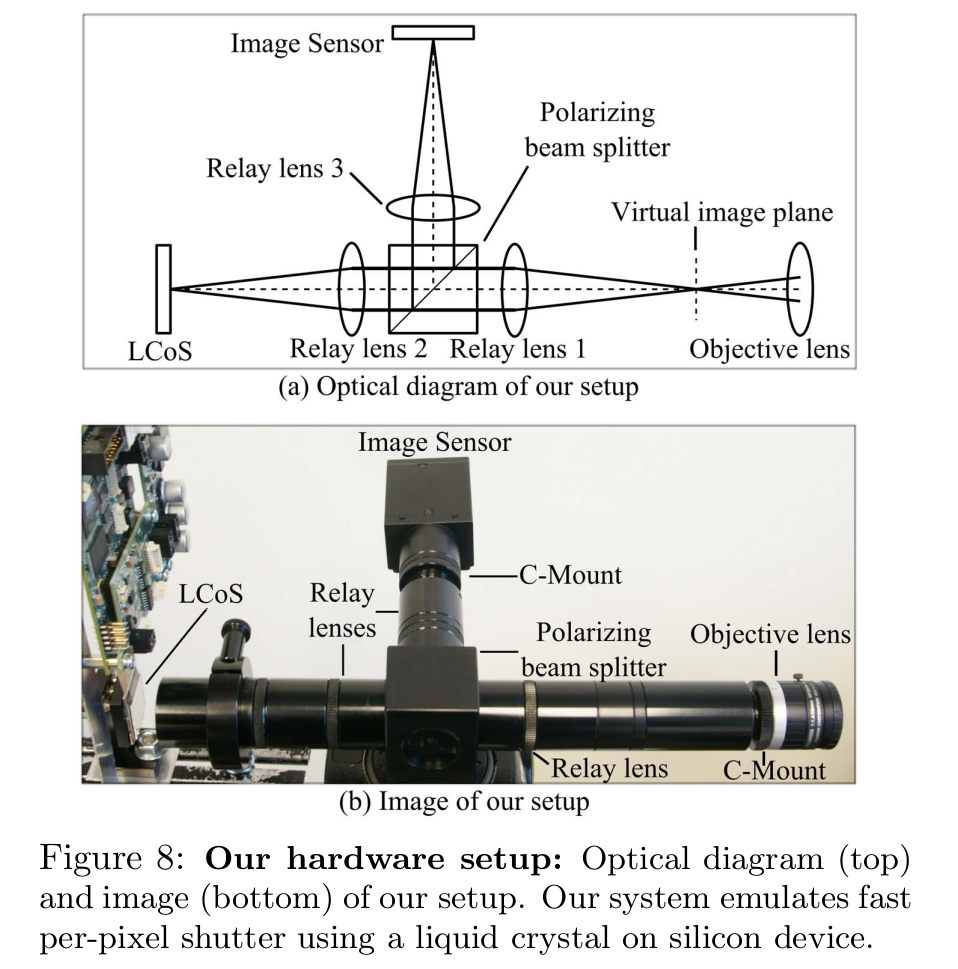
\includegraphics[scale=0.3]{hitomi.png}
        \caption{Hitomi et al paper' setup}
        \label{fig:hitomi}
\end{figure}

\medskip 

\begin{figure}[h!]
       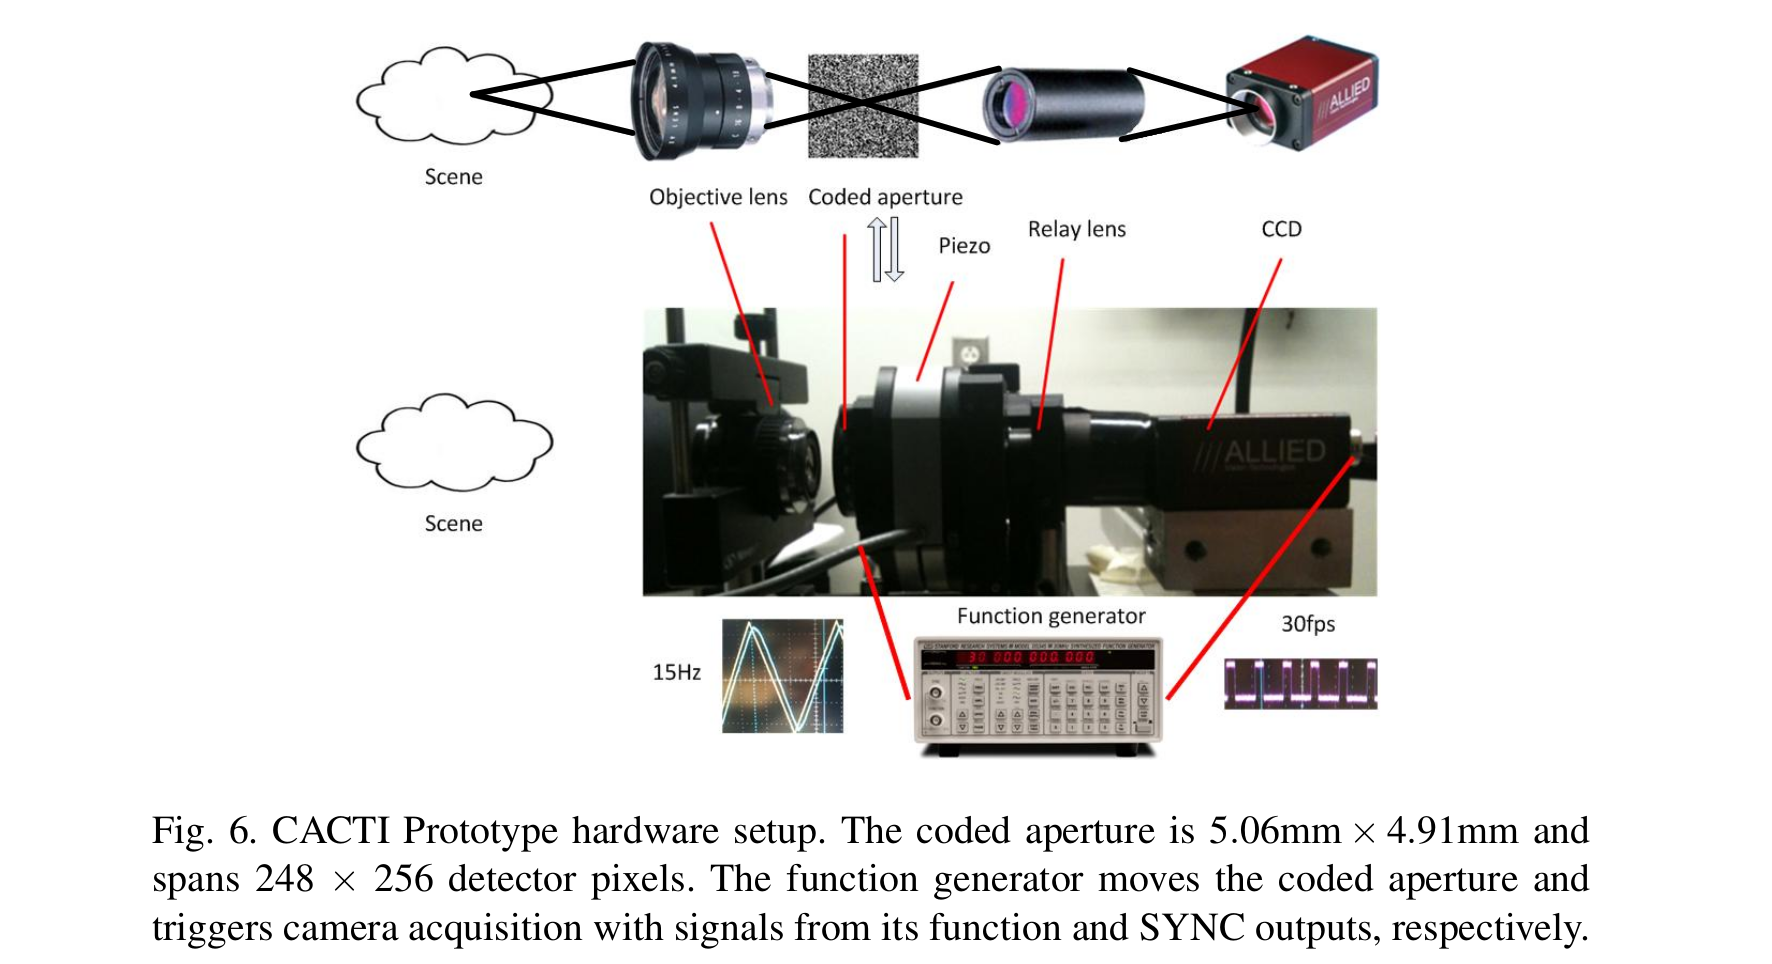
\includegraphics[scale=0.25]{duke.png}
       \caption{Duke University's paper's setup}
       \label{fig:duke}
\end{figure}


\subsubsection*{Similarities:}
\begin{enumerate}
    \item In both the set-ups, the scene is first imaged through a simple 
    objective lens before beginning with any complex processing. 
    \item Also, relay lens is used in both the cases for performing imaging of the 
    modulated scene on to the image sensor (e.g. a CCD Camera). 
    \item Structural sparsity of the sub-frames in each frame is supposed to be
    useful to reduce the measurements in both the set-ups.
    \item Hence, both the architectures are, in the end, supposed to save only the coded snapshots
    of each frame; which is later to be used for reconstruction. 
    \item The ``coding function" in both the architectures (i.e. called the coded aperture’s 
    transmission function in CACTI and known as the "sampling function" in the Hitomi et al 
    paper) uses random binary sampling.
    
\end{enumerate}



\subsubsection*{Differences:}
\begin{enumerate}
    \item Compressive measurement for visible imaging has been implemented using Liquid Crystal on
    Silicon (LCoS) devices to code pixel values incident on a single detector, in the Hitomi et al paper. LCoS is not used in CACTI.
    \item Instead of LCoS, CACTI proposes mechanical translation of a passive coded aperture for 
    the space-time compressive measurement.
    \item The LCoS strategy increases, rather than decreases, operating power and
    bandwidth. CACTI does low power space-time compressive measurement.
    \item Once imaged through an objective lens, the scene is first imaged 
    on a virtual image plane in Hitomi et al paper's setup. In the other one, the continuous scene f is directly imaged onto the piezo-positioned mask through an objective lens.
    \item The LCoS was operated at 1000 Hz. Such high frequencies are unheard of
    in the other setup. 
    \item Single bump exposure was essential in the Hitomi et al paper's setup. The coded aperture pattern in the other one didn't follow single bump exposure. 
\end{enumerate}


\newpage

\subsection*{(b) What cost function is the...}

Here, we'll explain the cost function used in the unconstrained optimization problem pertaining to the \textsf{Two-step Iterative-Shrinkage Thresholding} (TwIST) Algorithm.

TwIST solves the unconstrained optimization problem: 

\begin{center}
    $\mathbf{f_e}= \displaystyle \argmin_{\mathbf{f}}   \mathcal{C}(\mathbf{f}) $
\end{center}

Where, the cost function $\mathcal{C}(\mathbf{f})$ is:

\begin{center}
    $ \mathcal{C}(\mathbf{f}) = ||\mathbf{g - Hf} ||^2 + \lambda \Omega(\mathbf{f})$
\end{center}

\medskip 

Note: 

(i) \ $N$ is the total number of pixels in one frame. We suppose $\sqrt{N}$ pixels per row and per column.

(ii) $N_F$ is the total number of frames in one coded snapshot.

\medskip

Now we explain the meaning and dimensions of the terms in $\mathcal{C}(\mathbf{f})$:
$\mathbf{f}, \mathbf{g}, \mathbf{H},
\Omega(\mathbf{f}),$ and $ \lambda$ respectively.

\medskip


\begin{enumerate}


\item $\mathbf{f}$: This denotes the three-dimensional (2 spatial and 1 temporal) scene that we're trying to capture. $\mathbf{f}$ was originally 
the scene's discretized form, with $\mathbf{f} \in \mathbb{R}^{\sqrt{N} \times \sqrt{N} \times N_F }$. In the 
cost function, this $\mathbf{f}$ is flattened so that $\mathbf{f} \in \mathbb{R}^{N N_F \times 1}$. 

As we'll see later, in $\Omega(\mathbf{f})$, $f_{i,j,k}$ denotes the pixel value wrt the scene 
$\mathbf{f} \in \mathbb{R}^{\sqrt{N} \times \sqrt{N} \times N_F }$. 
$(i,j)$ are spatial indices and $k$ is the temporal index. 

\medskip

\item $\mathbf{g}$: This is the detector image $\mathbf{g} \in \mathbb{R}^{\sqrt{N} \times \sqrt{N}}$, obtained by 
integrating the $N_F$ temporal channels of $\mathbf{f}$, through a time-varying spatial transmission pattern. 
In the cost function, this $\mathbf{g}$ is flattened so that $\mathbf{g} \in \mathbb{R}^{N \times 1}$. 

We can actually write,  $\mathbf{g= Hf +n}$, where $\mathbf{H}$ is as explained below, and 
$\mathbf{n} \in \mathbb{R}^{n \times 1}$ represents
the flattened noise vector, 
representing the imaging noise.

\medskip

\item $\mathbf{H}$: This is the system's discrete forward matrix. It accounts for sampling factors
including the optical impulse response, pixel sampling function, and time-varying transmission
function.

\medskip

It is a 2-D representation of the 
3-D time-varying spatial transmission pattern $\mathbf{T} \in  \mathbb{R}^{\sqrt{N} \times \sqrt{N} \times N_F }$.

This uniquely codes each of the $N_F$ temporal channels of $\mathbf{f}$. 

\smallskip

Let \hspace{5pt} $\mathbf{H_k} := \text{diag} [T_{1,1,k} \; \; T_{2,1,k} \;\; \cdots \;\; T_{\sqrt{N},\sqrt{N},k}] $ 
    where $k=1,2, \ldots, N_F$.
    
    \smallskip
    
    Each $\mathbf{H_k} \in \mathbb{R}^{N \times N}$
    
\smallskip

Then, $\mathbf{H}$ is a concatenation of all $\mathbf{H_k} , k \in \{1, 2, \cdots , N_F \}$.

\smallskip

 \hspace{10pt}   $\mathbf{H} := [\mathbf{H_1} \; \;  \mathbf{H_2}  \; \; \cdots \; \; \mathbf{H_{N_F}}]$

\smallskip

Thus, $\mathbf{H} \in \mathbb{R}^{N \times N N_F} $.

\newpage 

\item $\Omega(\mathbf{f})$: This is a regularizer function, included in the cost function so as to penalise characteristics of the estimated $\mathbf{f}$ 
that would result in poor reconstructions.  

Here, we use the Total Variation (TV) regularizer function, defined as:

\begin{center}
    $\Omega(\mathbf{f}) = \displaystyle \sum_{k}^{N_F} \sum_{i,j}^{N} \sqrt{ (f_{i+1,j,k}-f_{i,j,k})^2 + (f_{i,j,k}-f_{i,j+1,k})^2  }$
\end{center}


Since many natural scenes are well-described by sparse gradients, 
this function was chosen which penalizes especially those estimates, which have sharp spatial gradients
as desired.

\item $\lambda$ : $\lambda \in \mathbb{R}$ is a scalar constant, known as regularization weight.

\begin{enumerate}
    \item It basically \textit{quantifies} how much importance should be given to the regularizer function over 
    other terms in the cost function.
    \item The regularization weight was chosen via experimental optimization over
    several test values $\lambda \in [0.3, 2]$.
    \item It was observed that a weight of $\lambda =1$ yielded in the clearest reconstructions. 
\end{enumerate}

 
  

\end{enumerate}

\newpage
\section*{Question 6}
\addcontentsline{toc}{section}{Question 6}
\setcounter{equation}{0}

\subsection*{(a)}
Title of paper - "Compressed Sensing Microscopy with Scanning Line Probes" \\
Published on 26th Sept 2019 at arXiv. \\
Link to the paper - \url{https://arxiv.org/pdf/1909.12342.pdf}.


\subsection*{(b)}
Image reconstruction from scanning chemical microscopic imaging (SECM) data measured by continuous line probe (CLP). \\
A CLP-SECM scan is setup by putting the sample on a rotational stage and locate the line probe at one side of sample. A single scan line is generated as follows: \\
The microscope firstly rotate its stage by preassigned angle, then followed by step-wise moving CLP to the other end of sample with constant step-size. \\
At each steps, CLP measures the current generated by electro-chemical reaction between sample and probe end.\\
A line scan is the collection of all measurements at all steps with sample rotation fixed at some given angle. Combining single line scans under different sample rotation angles gives the complete CLP-SECM scan.\\

\begin{figure}[H]
   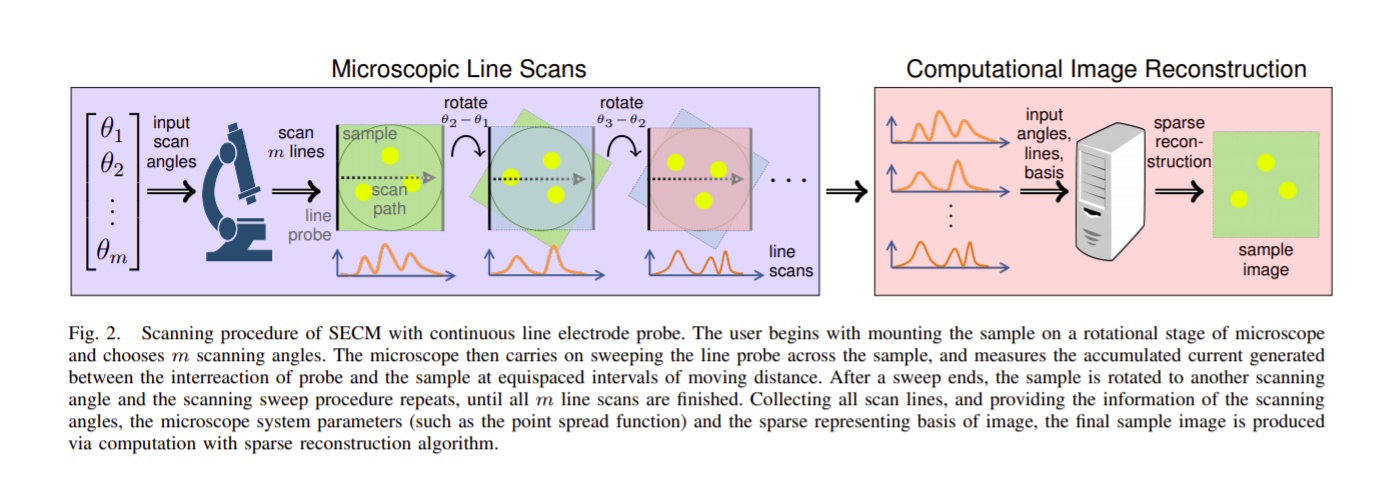
\includegraphics[scale=0.35]{Q6_Pg2.png}
   \caption{Page 2 of the paper - describes the basic flow of data}
\end{figure}
\begin{figure}[H]
   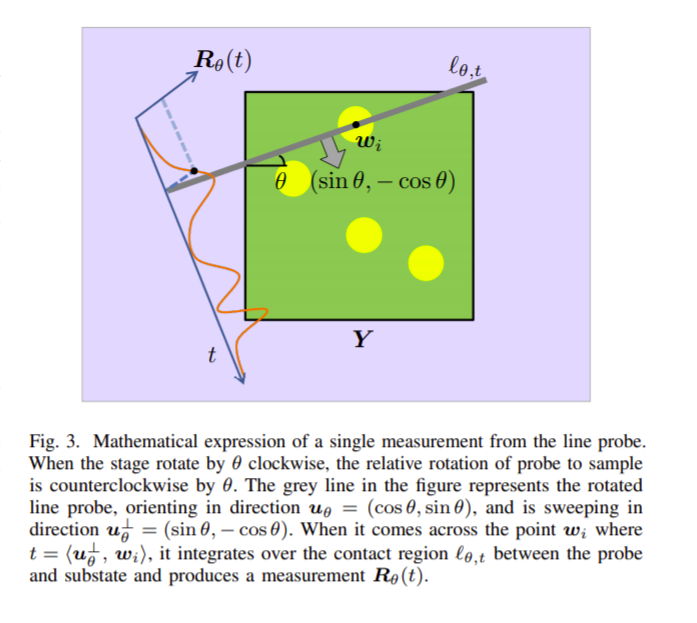
\includegraphics[scale=0.4]{Q6_Pg3.png}
  \caption{Page 3 of the paper - describes how the measurement of $R_\theta(t)$ is made}
\end{figure}
\begin{figure}[H]
   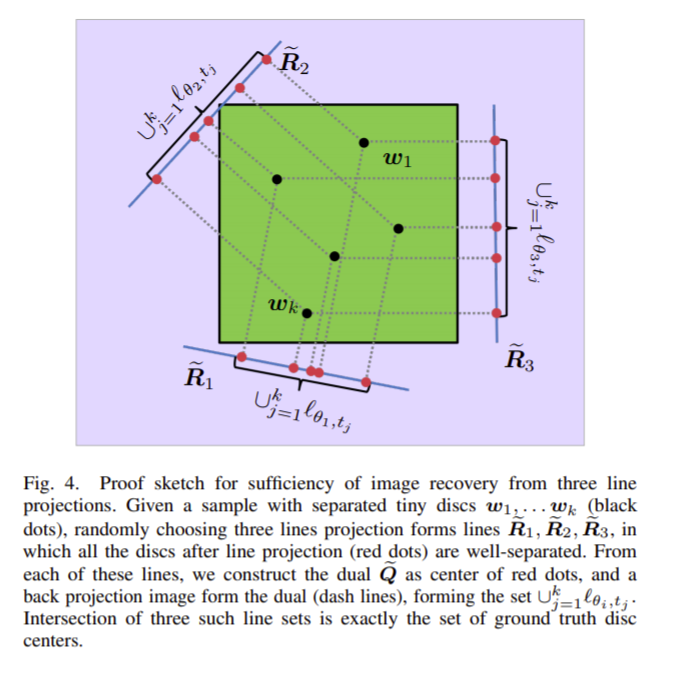
\includegraphics[scale=0.4]{Q6_Pg5.png}
   \caption{Page 5 of the paper - three line projections shown}
\end{figure}

\subsection*{(c)}
In the experiments performed, the interested sample---chemical reactive species attached on substrate is "highly structured". More specifically, the shape reactive species are known, are much smaller in comparison with the sample size, and also are sparsely populated on the substrate. \\
A sample Y can therefore being modeled as 2D-convolution between the reactive species $D$ and a sparse activation map $X_0$, denote as $Y = D * X_0$. We adopt \textbf{compressed sensing methodology}, to reconstruct the SECM sample image by finding the exact locations map $X_0$. Define CLP line scan $L$ takes the sample $Y$ and CLP properties $p$ -  scanning angles, point-spread function of CLP, etc., and generates measured current lines $R$ where $R = L[ D * X_0, p]$. \\

The reconstruction algorithm gathers CLP-SECM scan lines $R$ to perform image reconstruction using numerical optimization procedure. The algorithm formulate the task of finding the location of the reactive species as a variation of \textbf{LASSO problem}. Namely, the algorithm solves the following problem

$$\text{min}_{X>0, p} C||X||_1 + ||L[D*X-R, p]||^2$$

where $C$ is some positive constant, $||X||_1$ denotes total magnitude of $X$, and $||R||^2$ represents energy of lines $R$. We claim that the sample image reconstruction is successful, if the location (non-zero entries) of $X$ is identical to $X_0$.

\end{document}

